
%%%%%%%%%%%%%%%%%%%%%%%%%%%%%%%%%%%%
%{Background and Literature Review}%
%%%%%%%%%%%%%%%%%%%%%%%%%%%%%%%%%%%%
\section{Introduction}

%{summary for all the literature review}

%{ classification of motion models }
Techniques for autonomous vehicles in motion planning have been studied extensively in recent years \cite{motion_planning}. Various algorithms are developed for optimized and collision-free trajectories. However, these algorithms tends to assume the future trajectories of other agents to be known, while in fact we have only limited knowledge about how other surrounding vehicles will behave. Without in-traffic direct communications or high-level traffic commands, this over-simplified assumption will result in unrealistic and often over-cautious reaction to avoid collisions. In the following section, based on the method employed, motion prediction models are classified into three main categories : Physics-Based Models, Driver Behavior Models and Interactive Models.


\section{Physics-Based Models}
\label{Literature:Physics-Based}
Predicting surrounding vehicles' movements enables more active and more practical traffic studies. In the literature, physics-based motion predictions, as shown in Fig.~\ref{physics-based}, use dynamic or kinematic models governed by simple physics laws as surveyed in \cite{survey_motion_prediction}. These models requires less computational power, are easier to construct, and also have decent accuracy in short-term predictions\cite{physics_real_time, physics_velocity_obstacle}. Nevertheless, the original functions do not account for uncertainties in real traffic, as a result, have only limited ability to interact with other human drivers. Zhan et al. use  probability model of yielding/passing actions at a crossroad in the traffic optimization study in \cite{non-conservative}. Other prediction models such as the work of Ruf et al. \cite{sparc} use a cost map with probabilistic values on each path to optimize the global planner of vehicle movements. Despite Physics-Based Model are easy to be applied and demand low computational power, they still suffer from poor long-term predictions which means they are unable to anticipate the future paths of surrounding agents. In other words, there will be only minimum interaction between the ego vehicle and other traffic participants.

\begin{figure}[htbp]
\begin{center}
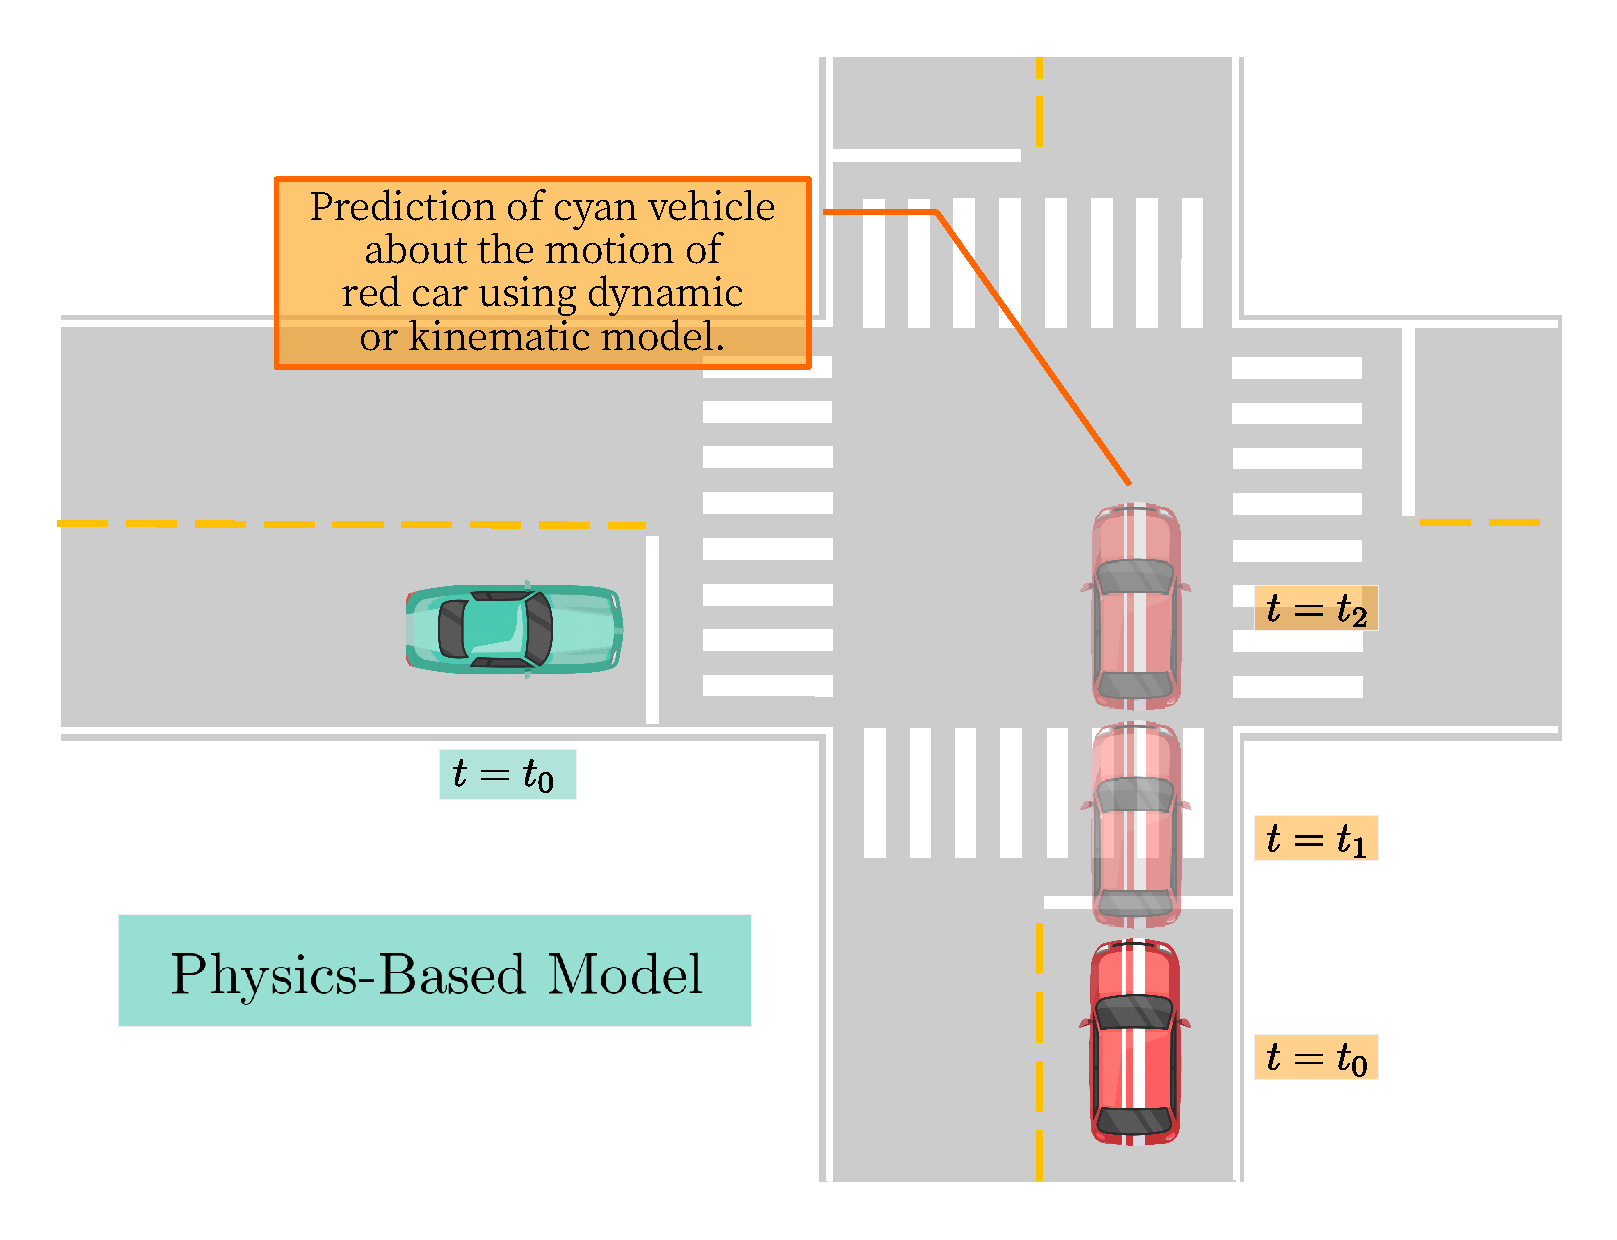
\includegraphics[scale=0.45]{intersection_physics.pdf}
\end{center}
\caption{Physics-Based Model.}
\label{physics-based} 
\end{figure}


\section{Driver Behavior Models}
\label{Literature:Driver Behavior}
A behavior could be a single action (e.g. braking, accelerating) or a series of actions (e.g. drive along a path require a series of actions). The motion prediction with Driver Behavior model is the intent recognition process based on the previous and current states of the target agent (as in Fig.~\ref{driver_behavior}). If the intent of the driver is identified, we can then predict the future behavior of the target vehicle. When handling the uncertainty of human behaviors, probabilistic method like Bayesian networks or Hidden Markov Model (HMM) are often used.

From the motion of the vehicle and the layout of the intersection, Lefevre et al. \cite{Lefevre2012} estimate the chance of a vehicle violating a stop sign with Dynamic Bayesian Network (DBN). In this work, the probability of the intention and expectation do not match is estimated. The intention stands for the intention to stop and the expectation is the necessity for the driver to stop given the circumstances (i.e. speed, turn signal and pose of the vehicle). Without the need to perform trajectory prediction, the proposed method is computationally efficient and flexible to different situations. 

Similar method is also used in literature where driver behaviors are predicted and recognized with DBN. Dagli et al. \cite{Dagli2003} construct a vehicle following and lane change models which form the basics for the behavior recognition. DBN is used to handle the uncertainty in sensor data gathering and human driver behaviors. The performance of this model is assessed in a simulated lane change experiment where the driver behaviors is recognized 1.5 seconds earlier than the actual lane change. Combining the manually formulated models and models learned with  random forest tree, Gindele et al. \cite{Gindele2013} use DBN to estimate and predict the driver behaviors of two cars passing the intersection. Online learning is possible in the proposed method where the model would be able to adapt to new environments.

\newpage

\begin{figure}[htbp]
\begin{center}
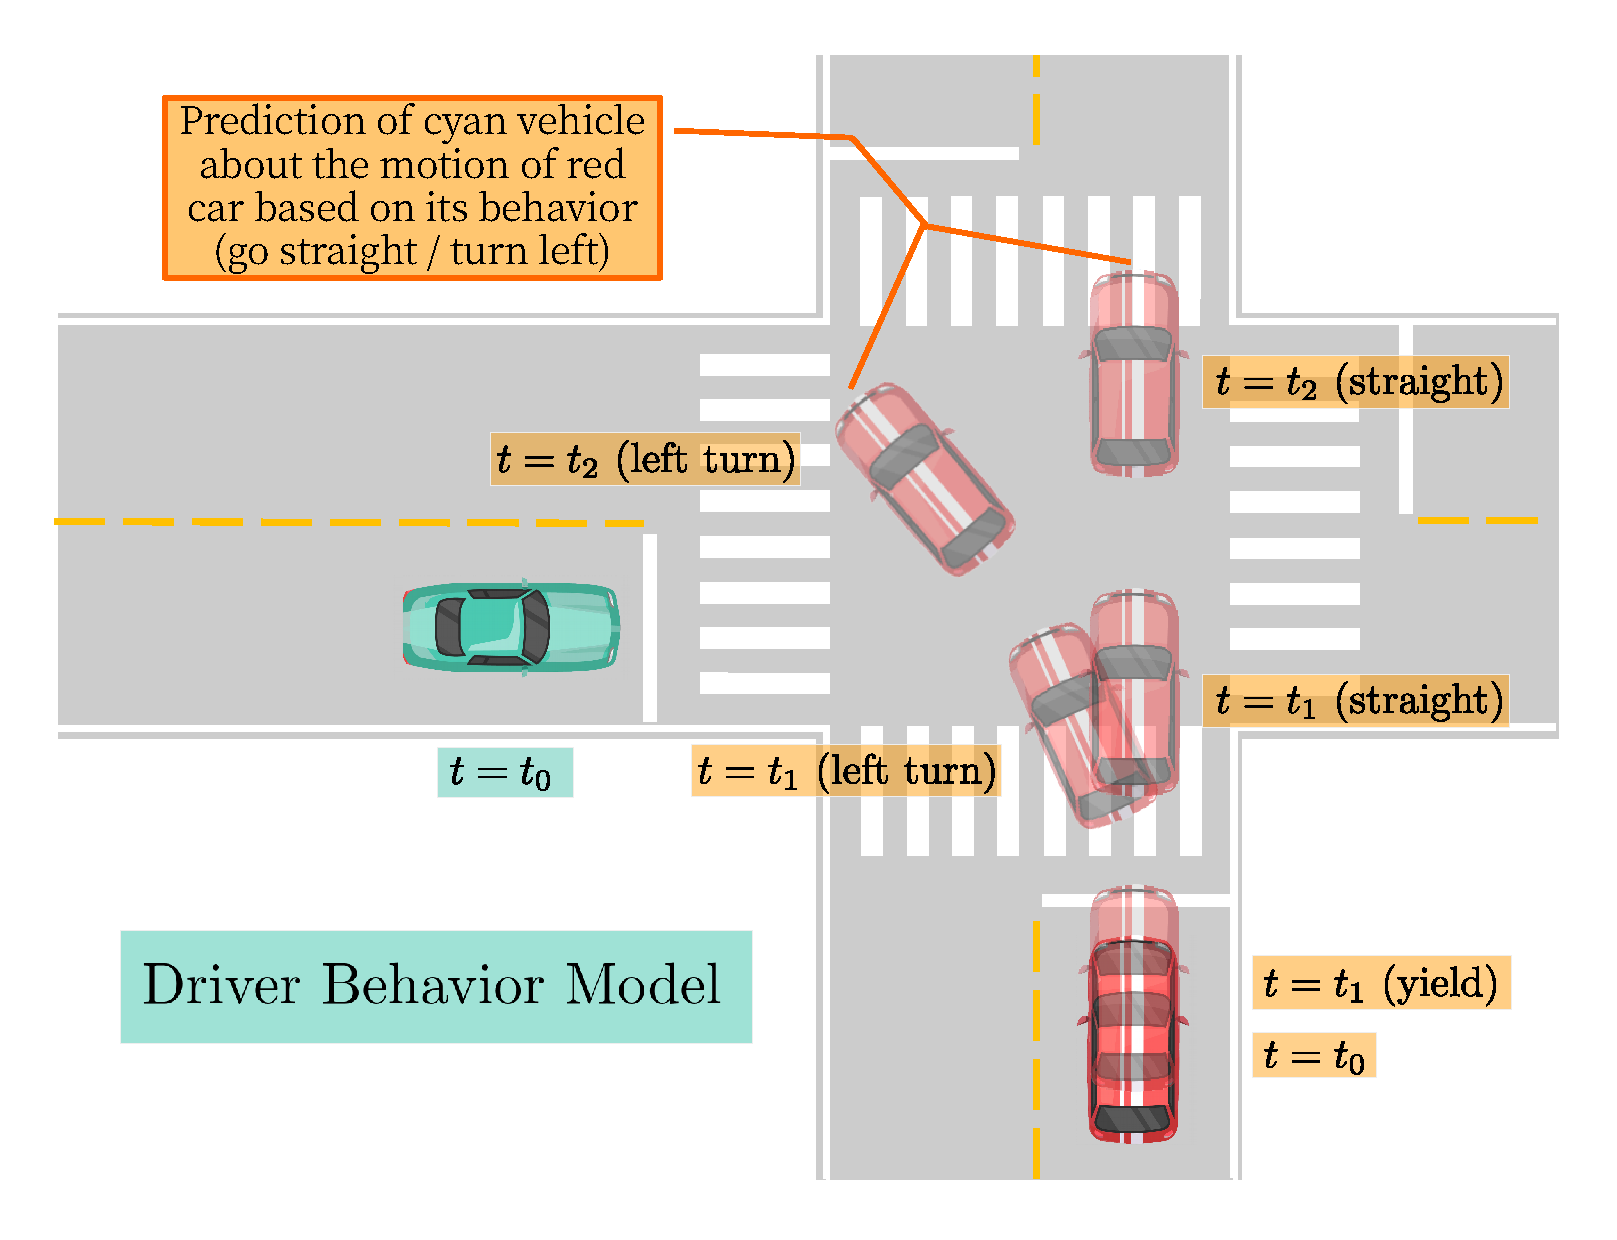
\includegraphics[scale=0.45]{intersection_behavior.pdf}
\end{center}
\caption{Driver Behavior Model.}
\label{driver_behavior} 
\end{figure}


\section{Interactive Models}
\label{Literature:Interactive}
To achieve a better long-term prediction while considering the joint behaviors between traffic participants, interactive models are used . In these models, all the motions and behaviors of a vehicle is considered having a causal relationship with surrounding agents (as in Fig.~\ref{interactive}). Hence a better behavior prediction or recognition results could be acquired. In order to generate interactive models, probabilistic methods such as partially observable Markov decision process (POMDP) have been applied.  POMDP can decide the actions of the host agent while interacting with other traffic participants by predicting their future states and taking their current state into account. Navigation and obstacle avoidance are solved in a probabilistic manner using POMDP by Foka et al. \cite{Foka}. Hubmann et al. \cite{state_uncertain_environment} also use POMDP to evaluate the possible maneuvers of other agents and optimize the actions of the host agent. Despite the advantages, POMDP is typically solved off-line, which means it's intractable for large state spaces. Its large demand for computational power also making it struggle to do the  prediction in real-time. Driver behavior models, on the other hand, have no need to predict the whole future trajectory of the target vehicle, thus are able to solve this problem. 


\begin{figure}[htbp]
\begin{center}
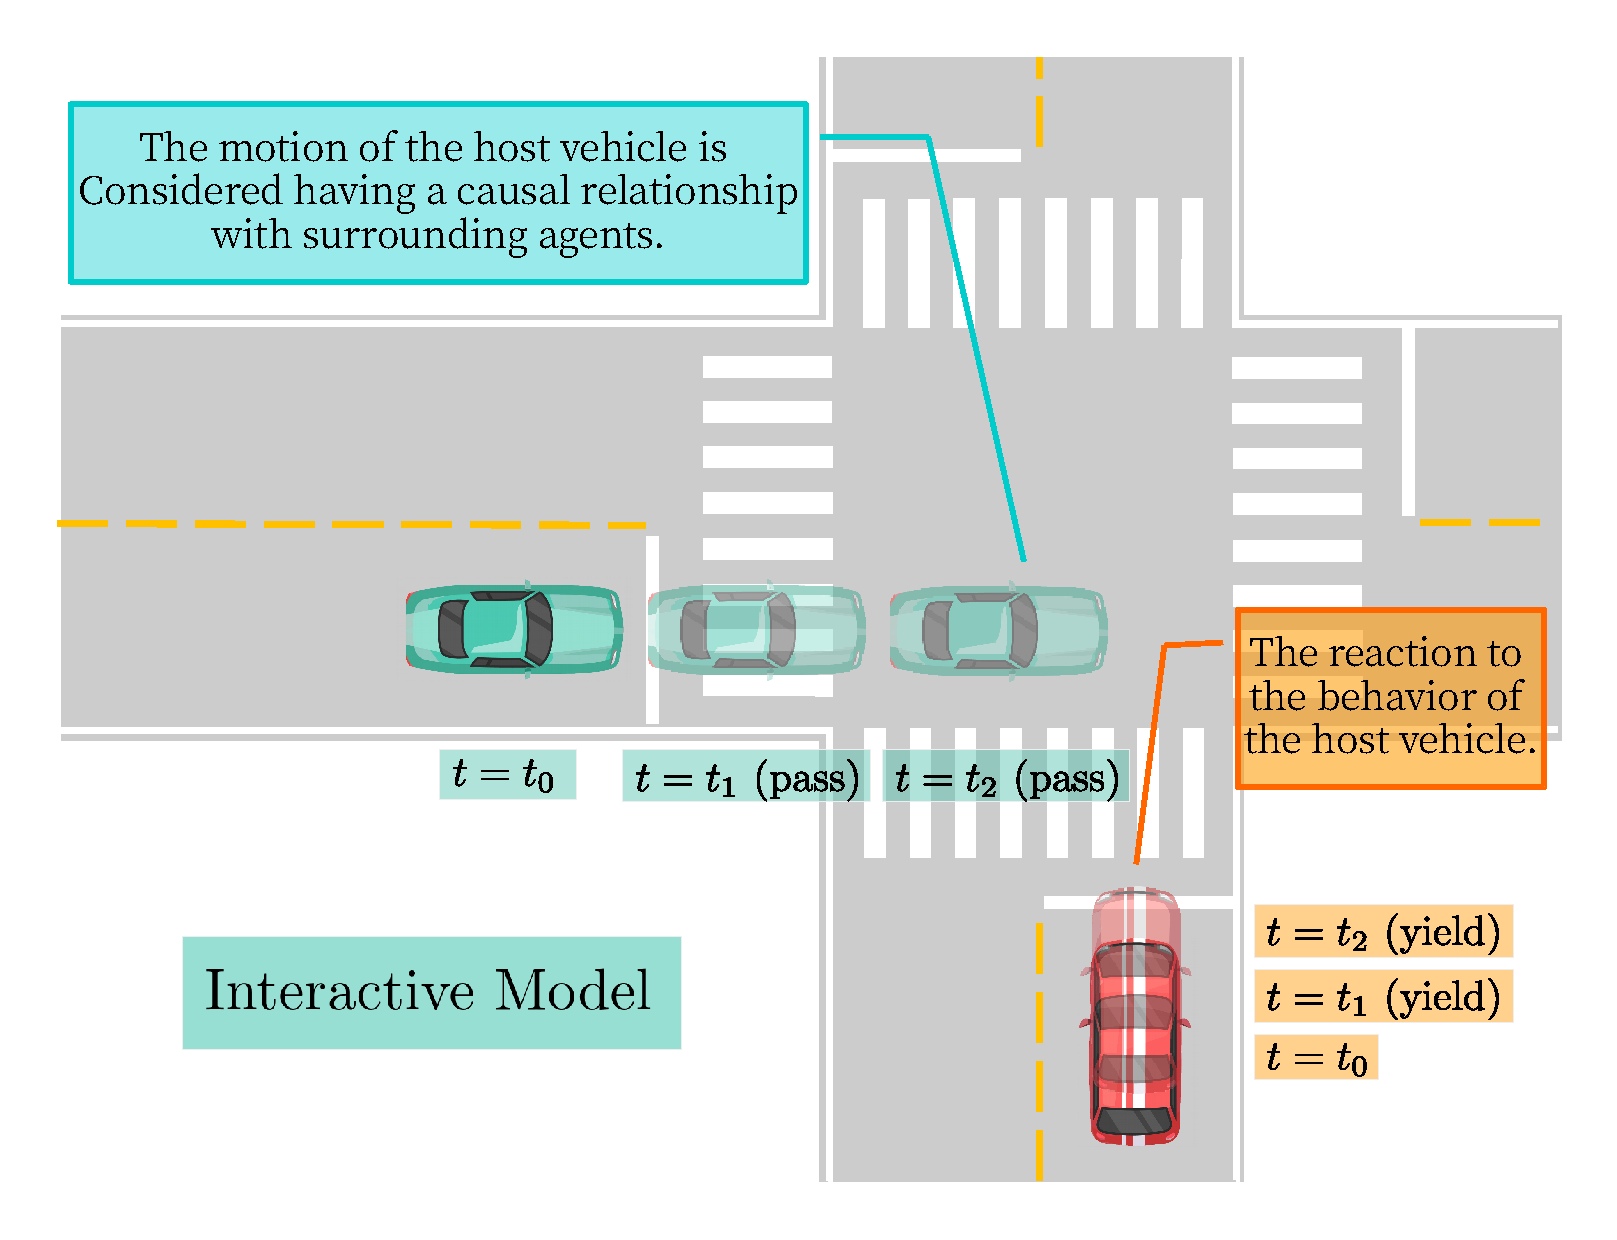
\includegraphics[scale=0.45]{intersection_interactive.pdf}
\end{center}
\caption{Interactive Model.}
\label{interactive} 
\end{figure}



\section{Explicit Driver Behavior Models}

Driver intent prediction for urban intersection has been a basic requirement for Advance Driver Assistance System (ADAS). To predict turn and stop maneuvers, Liebner et al. \cite{Liebner2012} use the Intelligent Driver Model (IDM) to model probability of turning and car-following behaviors in a simple Bayes net. The resulting probabilities of four different intentions are compared. The proposed method could be applied to arbitrary intersection if a more generalized desired velocity profiles are used.

For the purpose of overcoming the changing driver behavior at site-specific intersections, Graf et al. \cite{Graf2014} extract important features from participants (e.g. speed, distance to the intersection) then put them in the process of Case-Based Reasoning (CBR). The main idea of CBR is to identify a case from experience that is similar to the current one, and use the result to predict the behavior of the driver. However, the results learned from one intersection still do not perform well at other intersections. Drivers with different driving style also affect the prediction accuracy significantly.   

Despite the Driver Behavior Model has the advantage of better long-term estimation than Physics-Based Models as mentioned in \ref{Literature:Physics-Based} and better the computational efficiency than Interactive Models in \ref{Literature:Interactive}, most of the models using pre-trained model are only applicable to designated situations and environments where the training data is extracted. To overcome this problem, more general and explicit driver behavior models is needed.



\section{Summary}
Despite the explicit formulation and general applicability, physics-based models can not account for states changes of the subject, which results in the poor long-term prediction. Considering joint behaviors of surrounding agent, the interactive models do achieve a better long-term prediction, but they are computationally expensive and intractable for large state spaces. In this thesis, the driver behavior model is chosen for its better long-term prediction and computational efficiency compared to the other two models. Yet, being pre-trained models, most of the behavior models in the literature are restricted to specific traffic scenario or certain driving styles. Hence, in the following chapters, an explicit driver behavior models will be developed to account for driver behaviors at various traffic scenarios.

